\documentclass{jsarticle}
\usepackage[dvipdfmx]{graphicx}

\begin{document}
\title{技術資料:スピンドル冷却空気の送出系に関する計算}
\author{青木翔平}
\date{平成27年7月23日}

\section{スピンドル冷却系}

\begin{figure}[htbp]
 \centering
 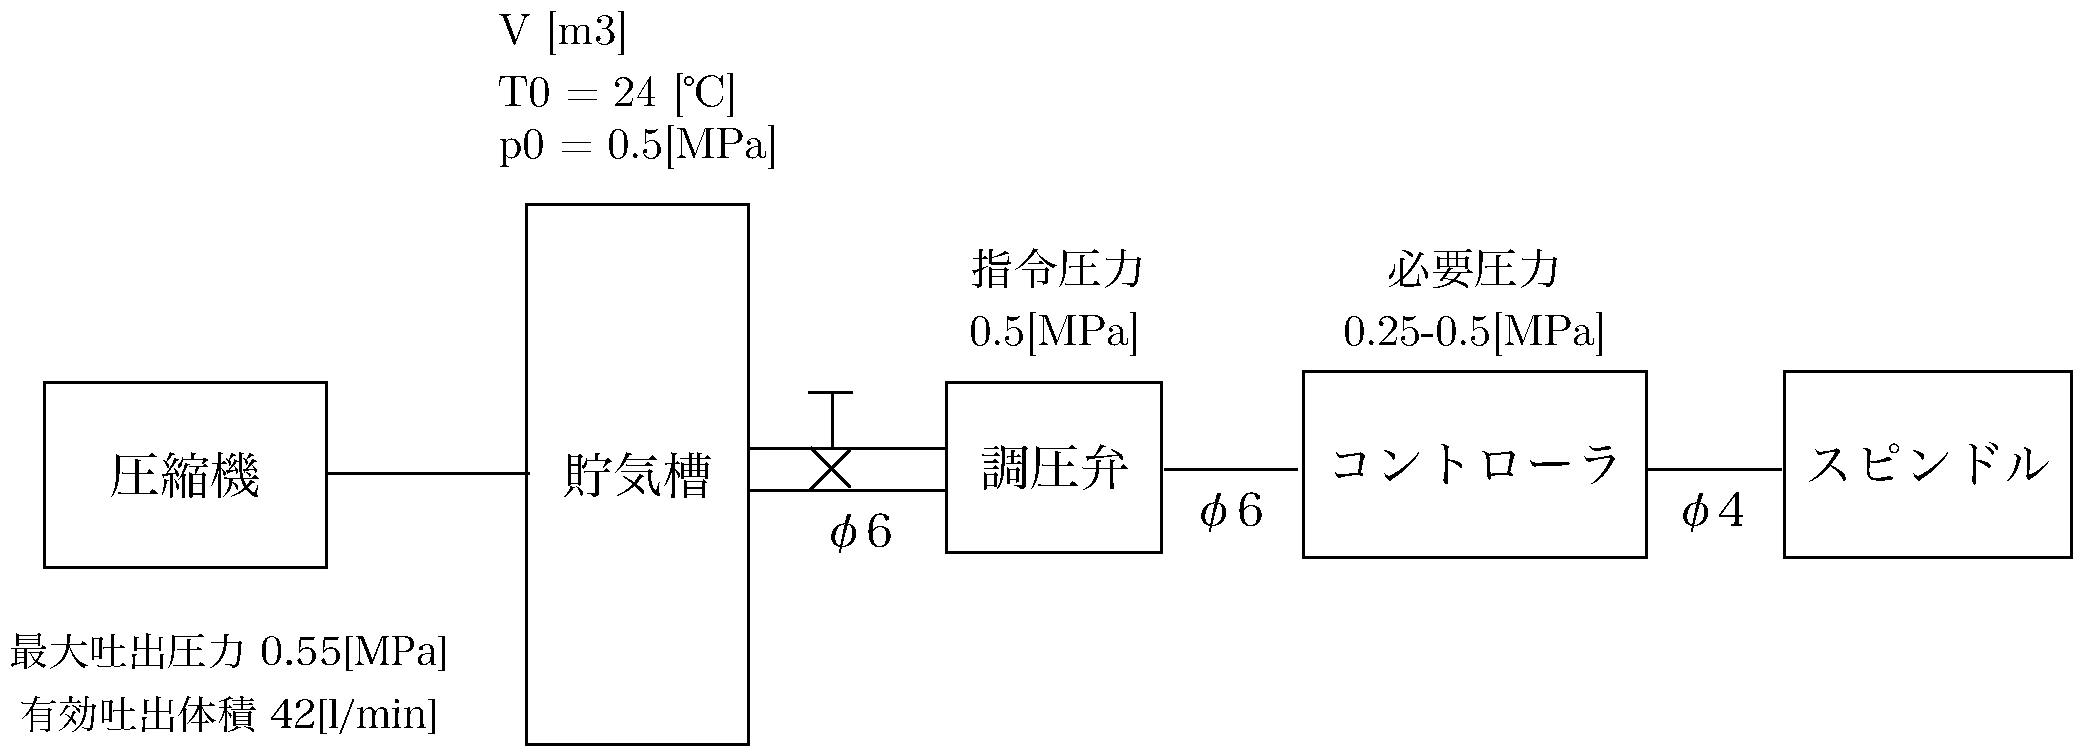
\includegraphics[width=150mm]{system.pdf}
 \caption{冷却システム構成図}
 \label{fig:solar_massage}
\end{figure}

\begin{eqnarray}
  \dot{m_c} & = &  \frac{P\dot{V_{s1}}}{RT}  \\
  \dot{m_d} & = & \frac{p_0 A_e }{\sqrt{R T}}\sigma^{*}
\end{eqnarray}

タンク内部の圧力を$p_0(t)$とおくと,流量の保存と気体の状態方程式から以下が成り立つ.
\begin{eqnarray}
  p_0(t) & = & \frac{R T_0}{V} \left( m_i + \dot{m_c} dt - \dot{m_d} dt \right) \nonumber \\
  & = & \frac{R T_0}{V} \left( \frac{p_a V}{R T_0} + \frac{p_a V_{s1}}{R T_0}dt - \frac{p_0(t) A_e}{\sqrt{R T_0}} \sigma^{*} dt \right) \nonumber \\
  & = & k_3 + k_2 dt - k_1 p_0(t) dt \label{eqn:diff} 
\end{eqnarray}
ただし,
\begin{eqnarray}
  k_1 & = & \frac{\sqrt{R T_0} A_e \sigma^{*}}{V}, k_2 = p_a \frac{V_{s1}}{V}, k_3 = p_{0i}
\end{eqnarray}
(\ref{eqn:diff})を微分して,
\begin{eqnarray}
  {p_0}^{\prime}(t) = k_2 - k_1 p_0(t)
\end{eqnarray}
$p_0(t)$を2次の項までテーラー展開して数値計算する.



\section{参考資料}
[1] 松尾 一泰, 「圧縮性流体力学―内部流れの理論と解析」, オーム社, 2013

\end{document}
